\section{{Resultados}}

En ambas instancias luego de la limpieza de los datos se finalizó con menos de
16 sujetos, descartando en el proceso aproximadamente 2 tercios de los ensayos
realizados (tabla \ref{{tab:clean-up-results}}).
Las figuras \ref{{fig:first-starting-sample-distribution}} y
\ref{{fig:second-starting-sample-distribution}} muestran la distribución de
ensayos según edad, frecuencia de muestreo y anchos de pantalla.
Se destaca la ausencia de sujetos de edad mayor a 50 años luego de aplicar los
criterios de filtrado.
Los pocos sujetos de tal grupo que sí realizaron el experimento (2 en la
primera ronda y 5 en la segunda) fueron en su mayoría descartados por obtener
una baja frecuencia de muestreo (figura \ref{{fig:sampling-frequencies-by-age}}).

\begin{{table}}[ht]
  \centering
  \begin{{tabular}}{{ c c | c | c }}
    \multicolumn{{2}}{{c}}{{ronda}} & primera & segunda \\ 
    \hline
    \multirow{{2}}{{10em}}{{pre-limpieza}}
      & sujetos
      & {first__starting_sample__subjects_count}
      & {second__starting_sample__subjects_count} \\  
      & ensayos
      & {first__starting_sample__trials_count}
      & {second__starting_sample__trials_count} \\  
    \hline
    \multirow{{2}}{{10em}}{{post-limpieza}}
      & sujetos
      & {first__inlier_sample__subjects_count}
      & {second__inlier_sample__subjects_count} \\  
      & ensayos
      & {first__inlier_sample__trials_count}
      & {second__inlier_sample__trials_count} \\  
    \hline
    \multirow{{2}}{{10em}}{{proporción conservada}}
      & sujetos
      & {first__kept_subjects_percentage}\%
      & {second__kept_subjects_percentage}\% \\  
      & ensayos
      & {first__kept_trials_percentage}\%
      & {second__kept_trials_percentage}\% \\  
  \end{{tabular}}

  \caption{{Ensayos pre y post limpieza}}
  \label{{tab:clean-up-results}}
\end{{table}}

\begin{{figure}}
  \centering

  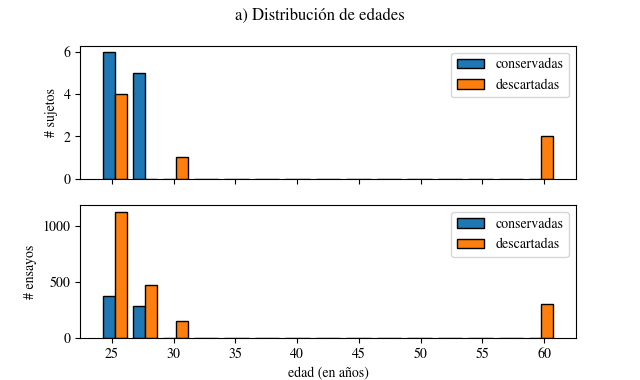
\includegraphics[width=0.8\linewidth]{{results/first-ages-distribution.png}}

  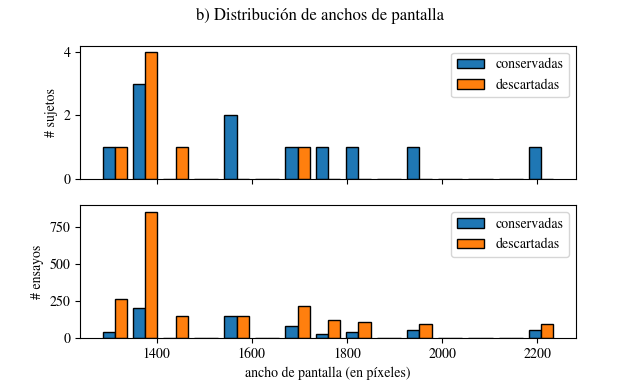
\includegraphics[width=0.8\linewidth]{{results/first-widths-distribution.png}}

  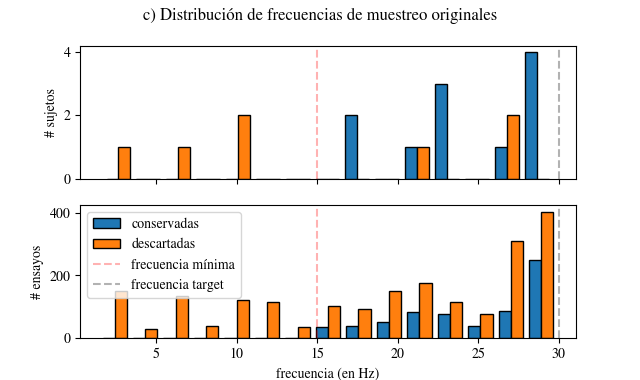
\includegraphics[width=0.8\linewidth]{{results/first-sampling-frequencies-distribution.png}}

  \caption{{Descripción general (primera instancia)}}
  \label{{fig:first-starting-sample-distribution}}
\end{{figure}}

\begin{{figure}}
  \centering

  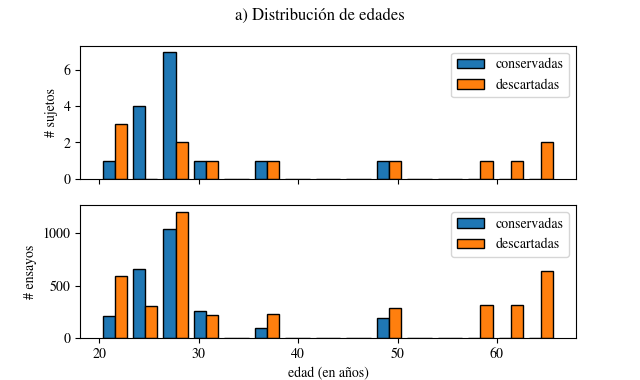
\includegraphics[width=0.8\linewidth]{{results/second-ages-distribution.png}}

  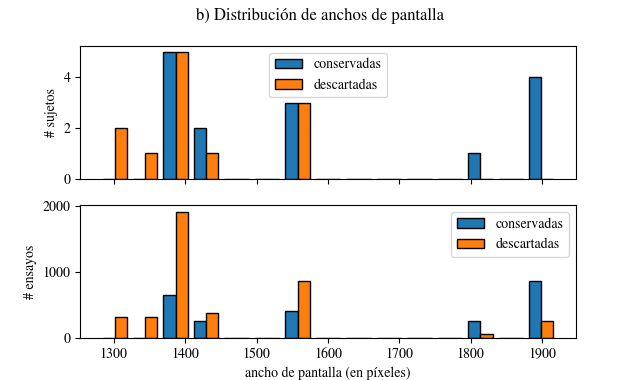
\includegraphics[width=0.8\linewidth]{{results/second-widths-distribution.png}}

  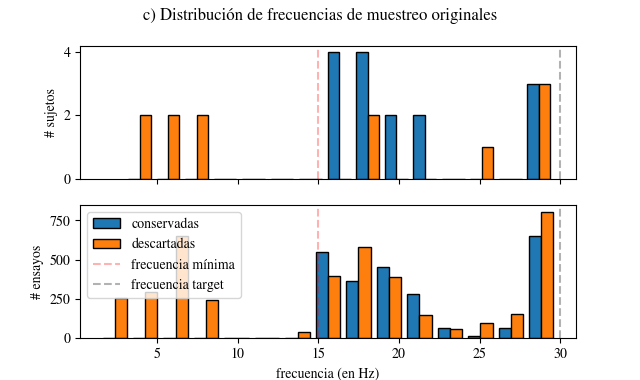
\includegraphics[width=0.8\linewidth]{{results/second-sampling-frequencies-distribution.png}}

  \caption{{Descripción general (segunda instancia)}}
  \label{{fig:second-starting-sample-distribution}}
\end{{figure}}

\begin{{figure}}
  \centering

  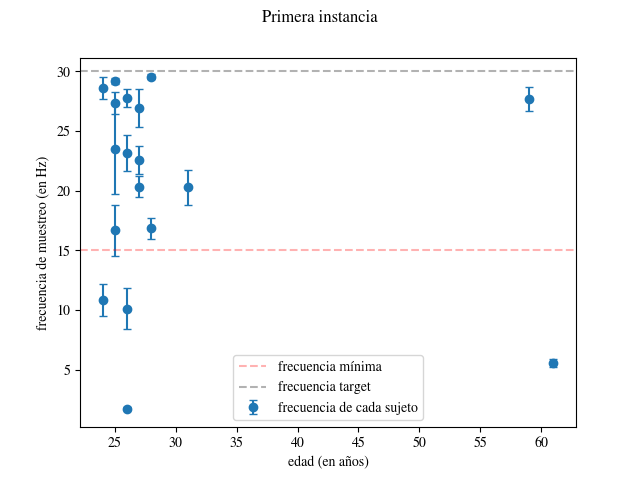
\includegraphics[width=0.9\linewidth]{{results/first-sampling-frequencies-by-age.png}}

  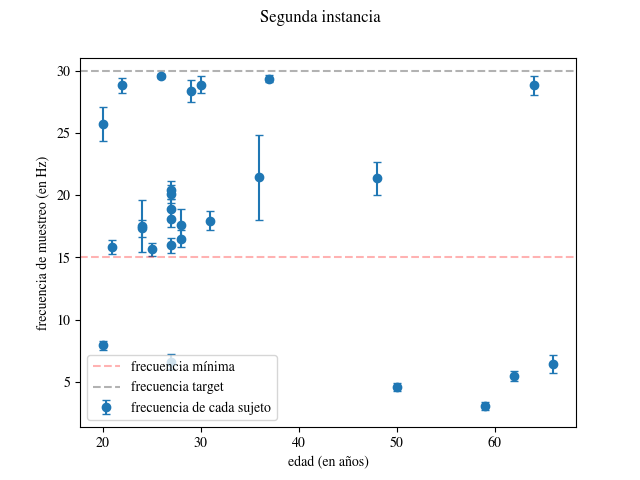
\includegraphics[width=0.9\linewidth]{{results/second-sampling-frequencies-by-age.png}}

  \caption{{Frecuencia de muestreo en función de la edad}}
  \label{{fig:sampling-frequencies-by-age}}
\end{{figure}}

Pudieron replicarse resultados generales esperados en la tarea de antisacadas.
Las antisacadas incorrectas mostraron tiempos de respuesta menores que las
antisacadas correctas.
Esto es consistente con la noción de que realizar correctamente la tarea
implica un costo cognitivo adicional.
En la primera instancia de experimentación se obtuvo, para la tarea de
antisacadas, una tasa de correctitud dentro del rango esperable.
Mientras que en la segunda fue mayor, pero sí se comportó como era esperado ya
que fue mayor para el caso prosacada que para antisacada.
Las tablas \ref{{tab:correcteness-rates}} y \ref{{tab:response-times}} así como
las figuras \ref{{fig:response-times-distribution}} y
\ref{{fig:response-times-distribution}} muestran el detalle de las
correctitudes y tiempos de respuesta obtenidos.
Las figuras \ref{{fig:first-disaggregated-prosaccades}},
\ref{{fig:second-disaggregated-antisaccades}} y
\ref{{fig:second-disaggregated-prosaccades}} muestran los ensayos obtenidos
clasificados según correctitud y tiempo de respuesta.

\begin{{table}}[ht]
  \centering
  \begin{{tabular}}{{c | c | c c}}
    ronda
      & primera
      & \multicolumn{{2}}{{c}}{{segunda}} \\
    tarea
      & antisacada
      & antisacada
      & prosacada \\
    \hline
    tasa de correctitud
      & {first__antisaccades_correctness_percentage}\%
      & {second__antisaccades_correctness_percentage}\%
      & {second__prosaccades_correctness_percentage}\% \\
  \end{{tabular}}
  \caption{{Tasas de correctitud}}
  \label{{tab:correcteness-rates}}
\end{{table}}

\begin{{table}}[ht]
  \centering

  \begin{{tabular}}{{ccc|c}}
          &       &             & tiempo de \\
    ronda & tarea & correctitud & respuesta (en ms) \\
          &       &             & \textit{{promedio (desvio std)}} \\
    \hline
    \multirow{{2}}*{{primera}}
      & \multirow{{2}}*{{antisacada}}
        & correcto
          & {first__correct_antisaccades_sample__mean_response_time}
            ({first__correct_antisaccades_sample__stdev_response_time}) \\
      &
        & incorrecto
          & {first__incorrect_antisaccades_sample__mean_response_time}
            ({first__incorrect_antisaccades_sample__stdev_response_time}) \\
    \hline
    \multirow{{4}}*{{segunda}}
      & \multirow{{2}}*{{antisacada}}
        & correcto
          & {second__correct_antisaccades_sample__mean_response_time}
            ({second__correct_antisaccades_sample__stdev_response_time}) \\
      &
        & incorrecto
          & {second__incorrect_antisaccades_sample__mean_response_time}
            ({second__incorrect_antisaccades_sample__stdev_response_time}) \\
      & \multirow{{2}}*{{prosacada}}
        & correcto
          & {second__correct_prosaccades_sample__mean_response_time}
            ({second__correct_prosaccades_sample__stdev_response_time}) \\
      &
        & incorrecto
          & {second__incorrect_prosaccades_sample__mean_response_time}
            ({second__incorrect_prosaccades_sample__stdev_response_time})
  \end{{tabular}}

  \caption{{Tiempos de respuesta}}
  \label{{tab:response-times}}
\end{{table}}

\begin{{figure}}
  \centering

  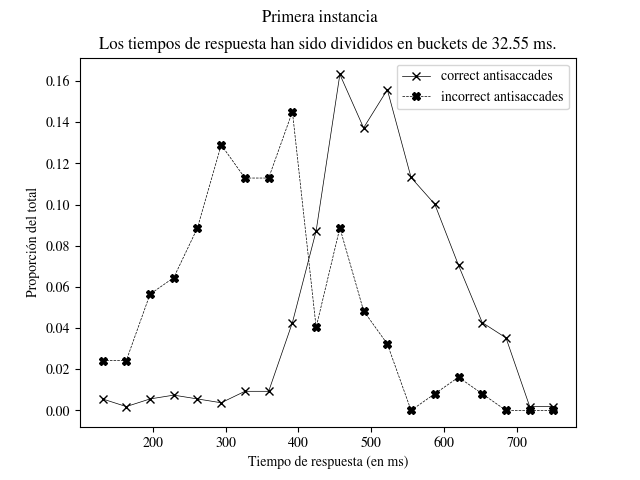
\includegraphics[width=0.9\linewidth]{{results/first-response-times-distribution.png}}

  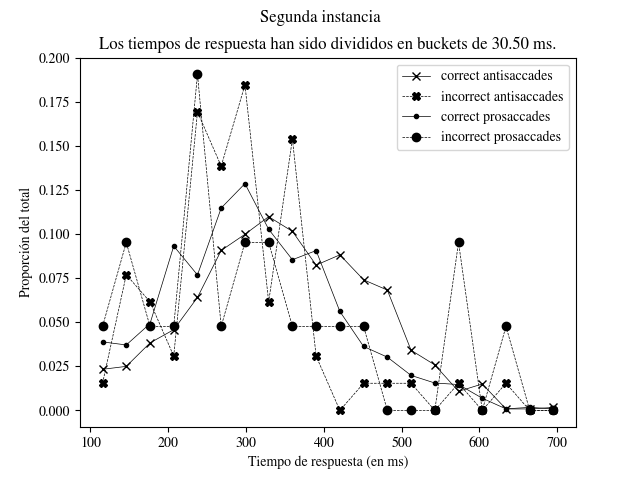
\includegraphics[width=0.9\linewidth]{{results/second-response-times-distribution.png}}

  \caption{{Distribución de tiempos de respuesta}}
  \label{{fig:response-times-distribution}}
\end{{figure}}

\begin{{figure}}
  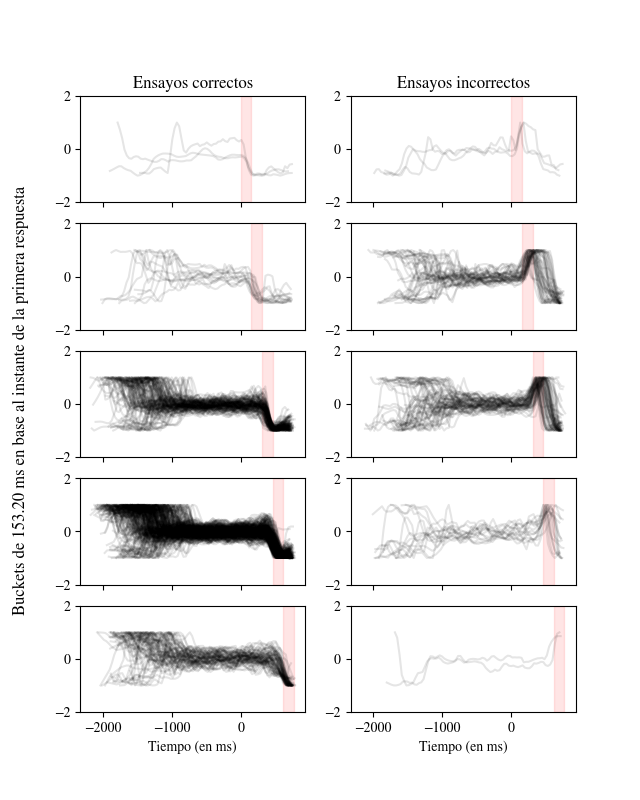
\includegraphics[width=\linewidth]{{results/first-disaggregated-antisaccades.png}}
  \caption{{Antisacadas desagregadas (primera instancia)}}
  \label{{fig:first-disaggregated-prosaccades}}
\end{{figure}}

\begin{{figure}}
  \centering
  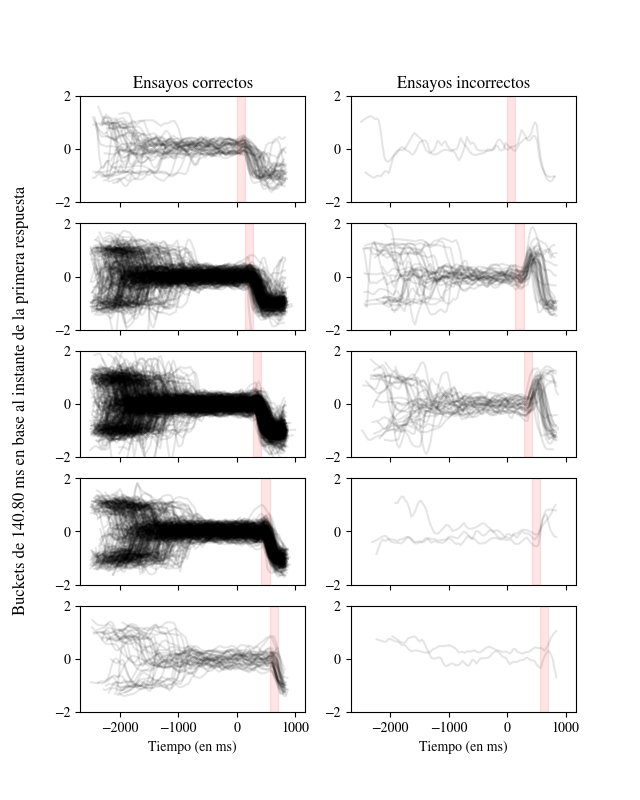
\includegraphics[width=\linewidth]{{results/second-disaggregated-antisaccades.png}}
  \caption{{Antisacadas desagregadas (segunda instancia)}}
  \label{{fig:second-disaggregated-antisaccades}}
\end{{figure}}

\begin{{figure}}
  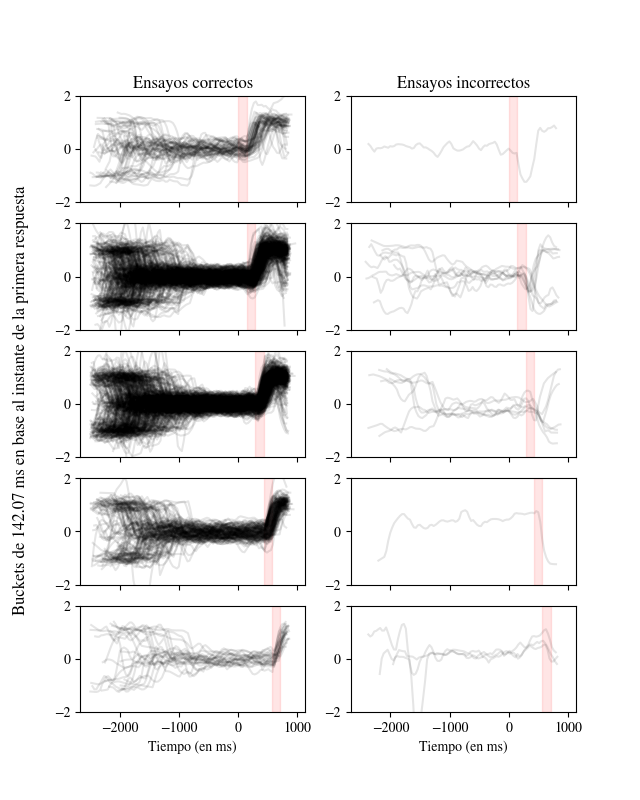
\includegraphics[width=\linewidth]{{results/second-disaggregated-prosaccades.png}}
  \caption{{Prosacadas desagregadas (segunda instancia)}}
  \label{{fig:second-disaggregated-prosaccades}}
\end{{figure}}

En ambos casos, en aproximadamente 80\% de los ensayos de antisacadas
incorrectas (tabla \ref{{tab:corrective-saccades}}) el sujeto realizó una
segunda sacada hacia la dirección correcta antes de la finalización del ensayo.
Esto es un indicio de que la tarea fue correctamente comprendida por los
sujetos.

\begin{{table}}[ht]
  \centering

  \begin{{tabular}}{{c|c|c}}
    ronda & primera & segunda \\
    \hline
    \# antisacadas incorrectas
      & {first__incorrect_antisaccades_sample__trials_count}
      & {second__incorrect_antisaccades_sample__trials_count} \\
    \# antisacadas corregidas
      & {first__corrected_antisaccades_sample__trials_count}
      & {second__corrected_antisaccades_sample__trials_count} \\
    \% de corrección
      & {first__antisaccades_correction_percentage}
      & {second__antisaccades_correction_percentage} \\
    tiempo de  & & \\
    corrección (en ms)
     &  {first__corrected_antisaccades_sample__mean_correction_delay}
       ({first__corrected_antisaccades_sample__stdev_correction_delay})
     &  {second__corrected_antisaccades_sample__mean_correction_delay}
       ({second__corrected_antisaccades_sample__stdev_correction_delay}) \\
    promedio (desvio std) & & \\
  \end{{tabular}}

  \caption{{Correcciones en las antisacadas incorrectas}}
  \label{{tab:corrective-saccades}}
\end{{table}}

En la segunda ronda, para todo sujeto se obtuvo una cantidad no significativa
de ensayos en ambos grupos incorrectos, algunos realizando incluso
correctamente todo sus ensayos
(tabla \ref{{tab:second-incorrect-count-per-subject}}).

{second__correctness_summary_table}
